\newpage
 \vspace{1.0cm}
 \headsep=1.5cm
 \centerline{\hei \sanhao 摘\ \ \ \ \ 要}
 \label{zhaiyao}
\vspace{0.5cm}
 \pagestyle{fancy}
 \fancyfoot[C]{---\thepage---}

这是华中师范大学物理科学与技术学院\textbf{非官方}硕士学位论文 \LaTeX 模板(官方只有 Word 模板),
理论上适用于所有专业。
原作者未知,若有人知晓,还望告知,我将正式征求授权和为其署名。

考虑到有人可能不熟悉 \LaTeX,
以及模板的流传范围太过狭窄,
我对其稍加修改,
私自上传到~\href{https://github.com/ichenh/ccnu-latex}{GitHub}~网站。
其中,我补充了更详细的说明,
添加了中文句号转换成英文句点命令,
增加了华师官方要求的论文(存档)封面,
将过期的 Hua-Zhong Normal University 图标换成了新的 Central China Normal University,
以及展示了一些基本的 \LaTeX 范例。
更详细的 \LaTeX 命令可参考 \CTeX 开发小组翻译的《\href{http://mirrors.ibiblio.org/CTAN/info/lshort/chinese/lshort-zh-cn.pdf}{一份(不太)简短的 \LaTeX $\ 2\varepsilon$介绍}》,
我将电子版放在了补充材料文件夹中,
其中也附上了华师官方的学位论文写作要求。
请随意使用和修改模板,欢迎补充,如有错漏,
还请在 GitHub 上提交 issue 或 Pull Request。

另外,建议使用 \href{https://ctan.org/mirrors/mirmon#cn}{TeX Live} 编译软件以及它自带的 TeXworks 编辑软件。
具体步骤是:

\begin{itemize}
\item[1] 修改论文封面:编辑根目录中的 ccnu-cover.doc 文件,另存为 ccnu-cover.pdf,覆盖原有文件。
\item[2] 打开 \verb!\include{/tex/}! 文件,按如下顺序进行排版生成 PDF 文件:XeLaTeX $\to$ BibTeX $\to$ XeLaTeX $\to$ XeLaTeX。
\item[3] 论文写作:打开 tex 文件夹,修改相应文件(对应于论文的不同部分和章节。
若要增加新的章节,复制一份 chapter2.tex,修改成 chapter3.tex,
在 main.tex 中的 \verb!\include{tex/chapter3}! 下方添加 \verb!\include{tex/chapter3}!。以此类推。
\item[4] 重复第二步,生成新的 PDF 文档。
\end{itemize}

整体思路很简单,由于论文一般很长,放在一个文件里不好整理,
所以分成多个文件,最后导入同一个文件中编辑。
根目录中的 \verb!\documentclass[12pt,a4paper]{article}
\usepackage{psfig,epsfig,graphicx,epstopdf}
\usepackage[UTF8]{ctex}
\usepackage{url}
\usepackage{IEEEtrantools}
  \usepackage{amsmath}
  \usepackage{amssymb}
  \usepackage{float}

% 由于论文一般比较长,为了方便查看,可以选择只编译 \includeonly{} 中的文件。
%\includeonly{tex/abstract,tex/chapter1,tex/chapter2,tex/appendix,tex/references,tex/toc}

\usepackage{indentfirst}
\usepackage[normal,footnotesize]{caption2}%%normal表示标题文本的格式是不足一行居中,多于左对齐;small是指标题号(如图..,表..)的字体大小。
\usepackage[sort]{cite}
\usepackage[top=3.9cm,bottom=3.5cm,left=2.8cm,right=3cm,headheight=1.2cm,footskip=0.8cm]{geometry}
\usepackage[colorlinks,linkcolor=black,anchorcolor=blue,citecolor=green]{hyperref}
\usepackage{pdfpages} % 插入pdf

%%%%%%%%%%%%%%%%%%%%%%%%
% 为了区分中文句号“。”和数学符号“o”,一般将其转换成英文句点“.”。
\catcode`\。=\active
\newcommand{。}{.}
%%%%%%%%%%%%%%%%%%%%%%%%

\makeatletter
\newcommand{\rmnum}[1]{\romannumeral #1}
\newcommand{\Rmnum}[1]{\expandafter\@slowromancap\romannumeral #1@}
\makeatother

%\textwidth=16.5cm
%\textheight=21.8cm
%\textwidth 14.3cm
%\textheight 19.9cm
%\oddsidemargin 1.2cm
%\oddsidemargin 1.2cm
%\evensidemargin 1.3cm
%\topmargin 0.3cm
%\headsep 25pt
%\hoffset=-28pt
%\voffset=-1.8cm
\def\baselinestretch{1.25}
\renewcommand{\theequation}%
  {\arabic{section}.\arabic{equation}}
  \renewcommand{\theequation}
  {\arabic{section}.\arabic{equation}}
\renewcommand{\thefigure}
  {\arabic{section}.\arabic{figure}}
\renewcommand{\thetable}
  {\arabic{section}.\arabic{table}}


\newcommand{\song}{\CJKfamily{song}} % 宋体 (Windows自带simsun.ttf)
\newcommand{\fs}{\CJKfamily{fs}} % 仿宋体 (Windows自带simfs.ttf)
\newcommand{\kai}{\CJKfamily{kai}} % 楷体 (Windows自带simkai.ttf)
\newcommand{\hei}{\CJKfamily{hei}} % 黑体 (Windows自带simhei.ttf)
\newcommand{\li}{\CJKfamily{li}} % 隶书 (Windows自带simli.ttf)
\newcommand{\you}{\CJKfamily{you}} % 幼圆 (Windows自带simyou.ttf)

\newcommand{\chuhao}{\fontsize{42pt}{\baselineskip}\selectfont} % 字号设置
\newcommand{\xiaochuhao}{\fontsize{36pt}{\baselineskip}\selectfont} % 字号设置
\newcommand{\yichu}{\fontsize{32pt}{\baselineskip}\selectfont} % 字号设置
\newcommand{\yihao}{\fontsize{26pt}{\baselineskip}\selectfont} % 字号设置
\newcommand{\erhao}{\fontsize{21pt}{\baselineskip}\selectfont} % 字号设置
\newcommand{\xiaoerhao}{\fontsize{18pt}{\baselineskip}\selectfont} % 字号设置
\newcommand{\sanhao}{\fontsize{15.75pt}{\baselineskip}\selectfont} % 字号设置
\newcommand{\sihao}{\fontsize{14pt}{\baselineskip}\selectfont} % 字号设置
\newcommand{\xiaosihao}{\fontsize{12pt}{\baselineskip}\selectfont} % 字号设置
\newcommand{\wuhao}{\fontsize{10.5pt}{\baselineskip}\selectfont} % 字号设置
\newcommand{\xiaowuhao}{\fontsize{9pt}{\baselineskip}\selectfont} % 字号设置
\newcommand{\liuhao}{\fontsize{7.875pt}{\baselineskip}\selectfont} % 字号设置
\newcommand{\qihao}{\fontsize{5.25pt}{\baselineskip}\selectfont} % 字号设置
%%%%%%%%%%%%%%%%%% 页眉与页脚 %%%%%%%%%%%%%%%%%%%%%%%%%%%%%%%%%%
\usepackage{fancyhdr,graphicx}
\newsavebox{\mygraphic}
\sbox{\mygraphic}{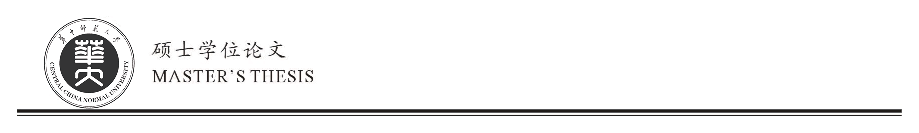
\includegraphics{logo.eps}}
\pagestyle{fancy}
\fancyhead{} % clear all header fields
\fancyhead[L]{\usebox{\mygraphic}}
\fancyfoot{} % clear all footer fields
\fancyfoot[C]{---\thepage---}
\renewcommand{\headrule}{%
\makebox[0pt][l]{\rule[0\baselineskip]{\headwidth}{0pt}}%
\rule[0\baselineskip]{\headwidth}{0pt} }

 %\renewcommand{\footrulewidth}{0.1pt}
 %\renewcommand{\headwidth}{\textwidth}


\begin{document}
\renewcommand{\refname}{\hei \sanhao 参考文献}
%%%%%%%%%%%%%%%%%%%%%%%%%%%%%%%%%%%%%%%%%%%%%%%%%%%%%%%%%%%%%%
%\
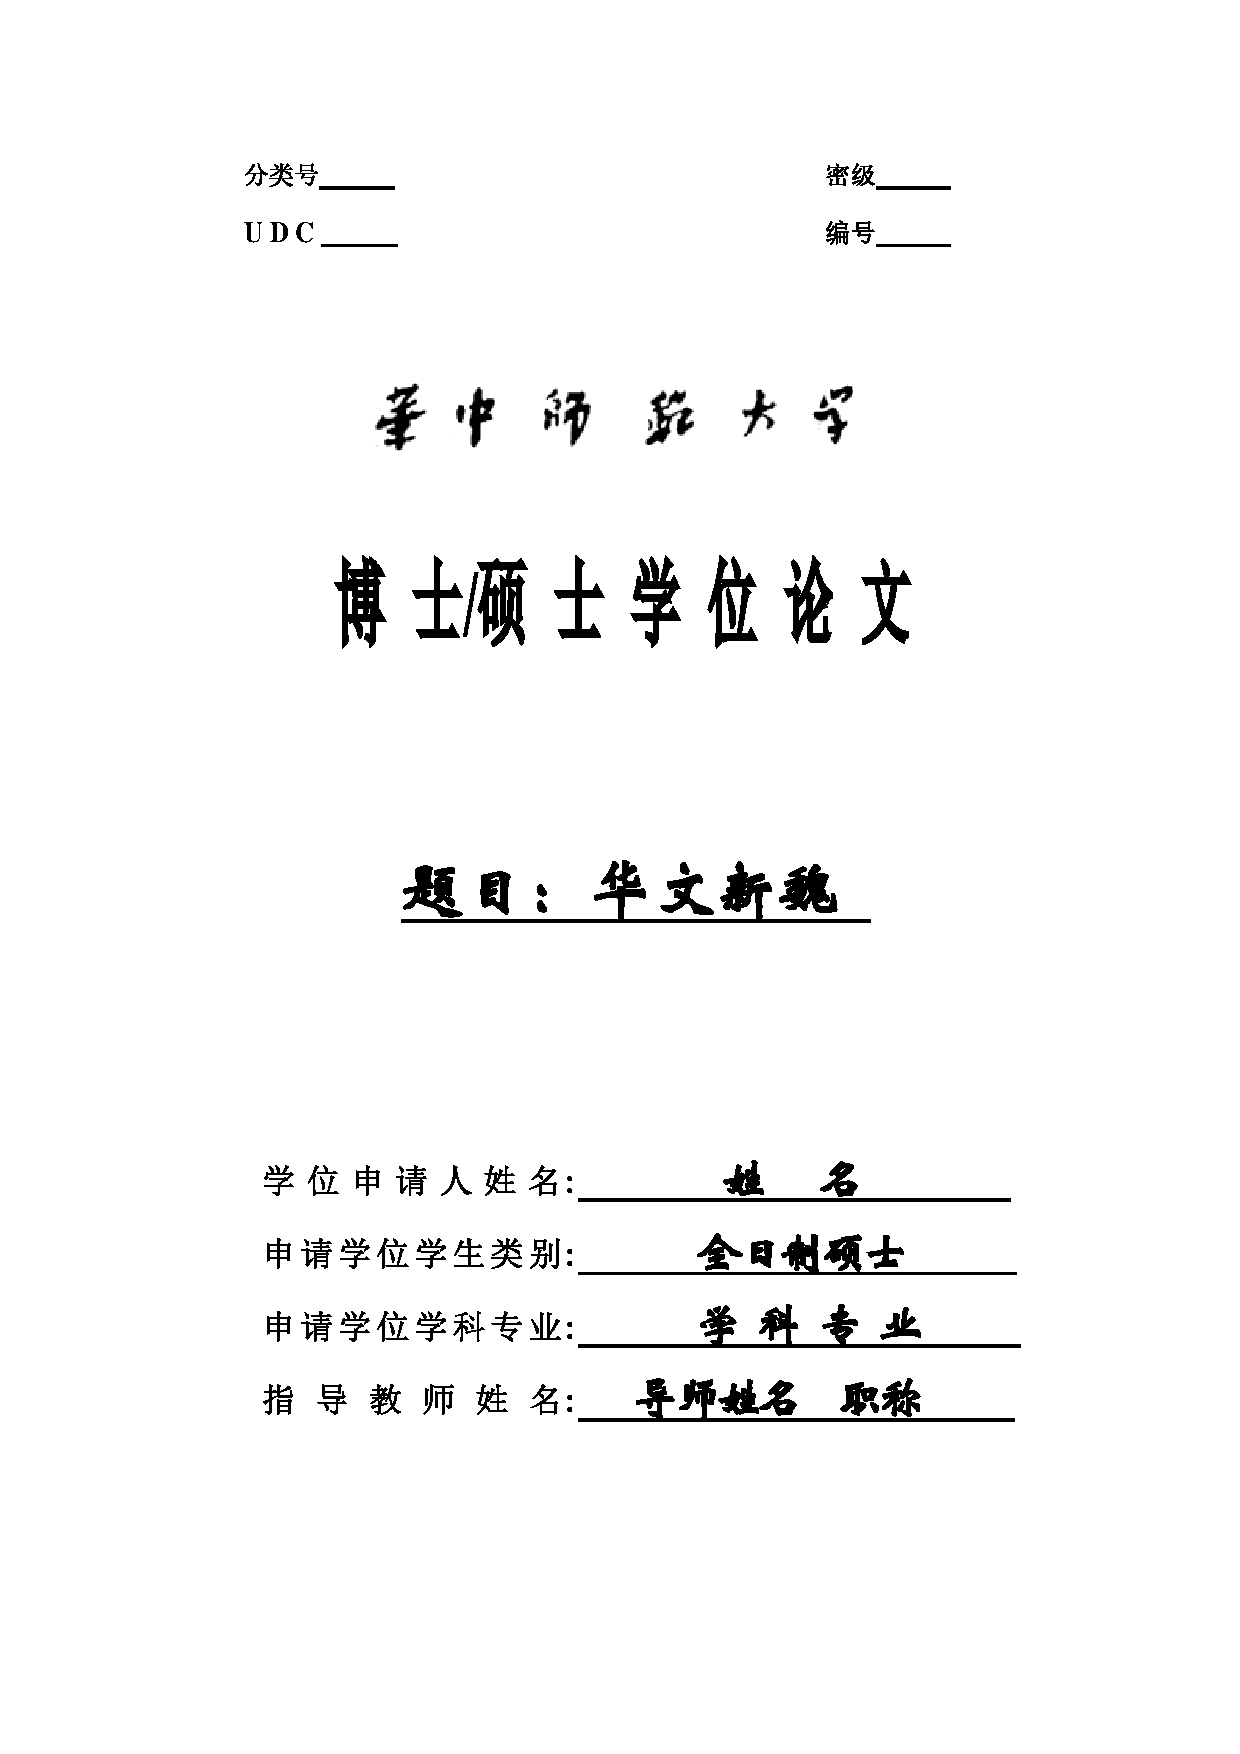
\includepdf{ccnu-cover.pdf} % 华师论文封面,在 ccnu-cover.doc 中修改,然后另存为 pdf 格式,替换掉模板
% 以下部分在 tex 文件夹中修改添加
% 标题页与授权页若不方便使用电子签名,可以先打印出来,签名后,扫描成 pdf 文件,按上述方法插入 tex 中
%%%%%%%%%%%%%%%%%%%% Chinese Cover %%%%%%%%%%%%%%%%%%%%%%%%%%%%%%%%%%%%%%%%%%%%
%\begingroup
%fancyfoot{} % clear all footer fields
%\thispagestyle{empty} %\markleft{\usebox{\mygraphic}}
\fancyfoot{}
\renewcommand{\thepage}{}
\begin{center}

%\hbox{} \vspace*{\fill}
\vspace*{2cm}
{\hei\yihao{{{\fontsize{28pt}{\baselineskip}\selectfont 硕士学位论文}}}}\\

\vspace*{2cm}

{\erhao \bf \hei 文章标题}\\


\vspace*{2.5cm}

\begin{huge}
\begin{center}
\begin{tabular}{cl}
  \xiaoerhao{\bf \hei 论文作者:}& \xiaoerhao{姓名} \\
  \xiaoerhao{\bf \hei 指导教师:}& \xiaoerhao{导师姓名\ 职称} \\
  \xiaoerhao{\bf \hei 学科专业:}& \xiaoerhao{专业名称} \\
  \xiaoerhao{\bf \hei 研究方向:}& \xiaoerhao{研究方向} \\
\end{tabular}
\end{center}
\end{huge}

\vspace*{3.5cm}

{\hei\xiaoerhao 华中师范大学物理科学与技术学院}

\vspace*{.5cm}

{\hei\xiaoerhao 2020年12月(修改时间)}

\vspace{\fill}
\end{center}

\newpage
%\endgroup

%%%%%%%%%%%%%%%%%%%% Second Cover %%%%%%%%%%%%%%%%%%%%%%%%%%%%%%%%%%%%%%%%%%%%
\newpage
%\begingroup
 \fancyfoot{} % clear all footer fields
%\thispagestyle{empty} %取消当前页码
\renewcommand{\thepage}{cover.en}
\begin{center}
%\hbox{} %\vspace*{\fill}

 \textbf{\xiaoerhao\bf \hei  论文英文标题}\\

 \vspace*{1.5cm}

{\large \sl A Thesis\\
\vspace*{0.4cm}
Submitted in Partial Fulfillment of the Requirements \\
\vspace*{0.4cm}For the Master's Degree in Astrophysics\\}

\vspace*{2cm}

{\normalsize\sanhao\hei\bf By}

\vspace*{0.4cm}

{\normalsize\sanhao\hei\bf 英文名}

\vspace*{0.4cm}

{\large \you \tt Postgraduate Program\\
\vspace*{0.4cm}
School of Physics and Technology\\
\vspace*{0.4cm} Central China Normal University\\}

\vspace*{2cm}

\textbf{\normalsize\sanhao\hei\bf Supervisor:
\hspace{1em}{\normalsize\sanhao\hei\bf  导师英文名}\hfill}

\vspace*{0.4cm}

\textbf{\normalsize\sanhao\hei\bf Academic Titles:
\hspace{1em}{\normalsize\sanhao\hei\bf 导师职称} \hfill}


\vspace*{0.5cm}

{\normalsize\sanhao \hfill Signature$\_ \_ \_ \_ \_ \_ \_ \_ \_ \_ \_ \_$}

\vspace*{0.3cm}

{\normalsize\sanhao \hfill Approved}

\vspace*{0.3cm}

{\normalsize\sanhao \hfill December, \hspace{0.5em}2020(修改时间)}

\vspace{\fill}

\end{center}
\newpage
%\endgroup
 % 标题页
%Authorization%%%%%%%%%%%%%%%%%%%%%%%%%%%%%%%%%%%%%%%%%%%%%%%%%%%
    \newpage
   %\thispagestyle{empty}
   \fancyfoot{} % clear all footer fields
    \begin{center}
    \title[\xiaoerhao {华中师范大学\\
    学位论文原创性声明和使用授权说明}
   \vspace{0.5cm}
    \parbox[t][1cm][c]{\textwidth}{ {\bf \sanhao \kai \centerline
    {原创性声明} } }
    \parbox[t][3cm][c]{\textwidth}{\xiaosihao
    \hspace{2em}本人郑重声明:所呈交的学位论文,是本人在导师指导下,独立
    进行研究工作所取得的研究成果。除文中已经标明引用的内容外,本论文不包含
    任何其他个人或集体已经发表或撰写过的研究成果。对本文的研究做出贡献的个
    人和集体,均已在文中以明确方式标明。本声明的法律结果由本人承担。}
    \parbox[t][2cm][c]{\textwidth}{\fontsize{12pt}{15pt}\selectfont
    \hspace{2em}\fs
    学位论文作者签名:
    \hspace*{3.3cm} 日期:\hspace{2em}年\hspace{2em}月\hspace{2em}日
    }

    \parbox[t][2cm][c]{\textwidth}{ {\sanhao \bf \kai \centerline
    {学位论文版权使用授权书} } }
    \parbox[t][3cm][c]{\textwidth}{\xiaosihao
    \hspace{2em}本学位论文作者完全了解学校有关保留、使用学位论文的规定,即:
    学校有权保留并向国家有关部门或机构送交论文的复印件和电子版,允许论文被查阅
    和借阅。本人授权华中师范大学可以将本学位论文的全部或部分内容编入有关数据库
    进行检索,可以采用影印、缩印或扫描等复制手段保存和汇编本学位论文。}
   \parbox[t][1.7cm][c]{\textwidth}{\fontsize{12pt}{15pt}\selectfont
   \hspace{2em}\fs
   学位论文作者签名:
   \hspace*{3.5cm}
   指导教师签名:}
   \parbox[t][1.8cm][c]{\textwidth}{\fontsize{12pt}{15pt}\selectfont
   \hspace{2em}\fs 日期:\hspace{2em}年\hspace{2em}月\hspace{2em}日
    \hspace*{2.3cm}日期:\hspace{2em}年\hspace{2em}月\hspace{2em}日
  \vspace{1.5cm}
}
 .\dotfill .
    \parbox[t][2cm][c]{\textwidth}{ {\fontsize{12pt}{18pt}\selectfont
    \hspace{2em}本人已经认真阅读"CALIS高校学位论文全文数据库发布章程",
    同意将本人的学位论文提交"CALIS高校学位论文全文数据库"中全文发布,
    并可按"章程"中的规定享受相关权益。同意论文提交后滞后:$\Box$半年;$\Box$一年;$\Box$二年发布。}}
   \parbox[t][1.5cm][c]{\textwidth}{\fontsize{12pt}{15pt}\selectfont
   \hspace{2em}\fs
   学位论文作者签名:
   \hspace*{3.5cm}
   指导教师签名:}
   \parbox[t][0.4cm][c]{\textwidth}{\fontsize{12pt}{15pt}\selectfont
   \hspace{2em}\fs 日期:\hspace{2em}年\hspace{2em}月\hspace{2em}日
    \hspace*{2.3cm}日期:\hspace{2em}年\hspace{2em}月\hspace{2em}日
    }
    \end{center} % 授权页
\pagenumbering{roman}
\newpage
 \vspace{1.0cm}
 \headsep=1.5cm
 \centerline{\hei \sanhao 摘\ \ \ \ \ 要}
 \label{zhaiyao}
\vspace{0.5cm}
 \pagestyle{fancy}
 \fancyfoot[C]{---\thepage---}

这是华中师范大学物理科学与技术学院\textbf{非官方}硕士学位论文 \LaTeX 模板(官方只有 Word 模板),
理论上适用于所有专业。
原作者未知,若有人知晓,还望告知,我将正式征求授权和为其署名。

考虑到有人可能不熟悉 \LaTeX,
以及模板的流传范围太过狭窄,
我对其稍加修改,
私自上传到~\href{https://github.com/ichenh/ccnu-latex}{GitHub}~网站。
其中,我补充了更详细的说明,
添加了中文句号转换成英文句点命令,
增加了华师官方要求的论文(存档)封面,
将过期的 Hua-Zhong Normal University 图标换成了新的 Central China Normal University,
以及展示了一些基本的 \LaTeX 范例。
更详细的 \LaTeX 命令可参考 \CTeX 开发小组翻译的《\href{http://mirrors.ibiblio.org/CTAN/info/lshort/chinese/lshort-zh-cn.pdf}{一份(不太)简短的 \LaTeX $\ 2\varepsilon$介绍}》,
我将电子版放在了补充材料文件夹中,
其中也附上了华师官方的学位论文写作要求。
请随意使用和修改模板,欢迎补充,如有错漏,
还请在 GitHub 上提交 issue 或 Pull Request。

另外,建议使用 \href{https://ctan.org/mirrors/mirmon#cn}{TeX Live} 编译软件以及它自带的 TeXworks 编辑软件。
具体步骤是:

\begin{itemize}
\item[1.] 修改论文封面:编辑根目录中的 \verb!ccnu-cover.doc! 文件,另存为 \verb!ccnu-cover.pdf!,覆盖原有文件。
\item[2.] 打开 \verb!main.tex! 文件,按如下顺序进行排版生成 \verb!main.pdf! 文件:XeLaTeX $\to$ BibTeX $\to$ XeLaTeX $\to$ XeLaTeX。
\item[3.] 论文写作:打开 tex 文件夹,修改相应文件(对应于论文的不同部分和章节。
若要增加新的章节,复制一份 \verb!chapter2.tex!,修改成 \verb!chapter3.tex!,
在 \verb!main.tex! 中的 \verb!\include{tex/chapter3}! 下方添加 \verb!\include{tex/chapter3}!。以此类推。
\item[4.] 重复第二步,生成新的 \verb!main.pdf! 文件。
\end{itemize}

整体思路很简单,
由于论文一般很长,放在一个文件里不好整理,
所以分成多个文件,最后导入同一个文件中编辑。
根目录中的 \verb!main.tex! 就是主要文件,只需编译它即可。
至于目录、引言、正文、参考文献等内容则分别放在 tex 目录下,
然后在 \verb!main.tex! 文件中通过 \verb!\include{}! 命令导入。

第二步中的 XeLaTeX 负责编译中文文本,BibTeX 是编译 \verb!.bib! 格式的参考文献。
若是使用了论文管理软件,可以选择导出为 \verb!.BibTeX! 文件,
覆盖 tex 文件夹下的 \verb!references.bib! 文件。
或者自己搜索相关文献的 BibTeX 引用格式,
将其复制到 tex 目录下的 \verb!references.bib! 文件中。
通过 BibTeX 编译出参考文献之后就只需要选择 XeLaTeX 编译,除非增加了新的文献。

\vspace{1cm} \noindent {\sihao \hei \textbf{关键词:}}华中师范大学;物理科学与技术学院;硕博士论文模板



\newpage %\vspace{1.5cm}
\headsep=0.7cm
\centerline{\bf \sanhao Abstract}
\label{abs}
\vspace{0.5cm}

Emmm...

\vspace{1cm} \noindent {\sihao \textbf{Keywords: }}CCNU; College of Physical Science and Technology; Tempolate of Doctoral or Master thesis % 摘要
\newpage
\pagestyle{fancy}
\thispagestyle{empty}
 %\fancyfoot{}
 \vspace{1.0cm}
 \centerline{\hei \sanhao 目\ \ \ \ \ 录}
\vspace{0.5cm} \label{content} \noindent
{\hei \xiaosihao 摘要 \dotfill \pageref{zhaiyao}}\\[0.2cm]
{\hei \xiaosihao ABSTRACT \dotfill \pageref{abs}}\\[0.2cm]
%{\hei \xiaosihao 目录\dotfill \pageref{content}}\\[0.2cm]
{\hei \xiaosihao 第一章\ \ \ \ 引言 \dotfill \pageref{1}}\\[0.2cm]
\hspace*{0.5cm} \ \  \ 1.1\ \  第一节\dotfill \pageref{1.1}\\
\hspace*{0.5cm} \ \  \ 1.2\ \  第二节\dotfill \pageref{1.2}\\[0.2cm] % 每章末尾添加 [0.2cm]
{\hei \xiaosihao 第二章\ \ \ \ \LaTeX 举例 \dotfill \pageref{2}}\\[0.2cm]
\hspace*{0.5cm} \ \  \ 2.1\ \  宇宙学标准模型\dotfill \pageref{2.1}\\
\hspace*{0.5cm} \ \  \ 2.2\ \  粒子物理标准模型\dotfill \pageref{2.2}\\[0.2cm]
{\hei \xiaosihao 第三章\ \ \ \ 总结与展望 \dotfill \pageref{3}}\\[0.2cm]
{\hei \xiaosihao 附录A\ \ \ \ 附录A \dotfill \pageref{A}}\\
\hspace*{0.5cm} \ \  \ A.1\ 通过 GitHub 写论文\dotfill \pageref{A.1}\\[0.2cm]
{\hei \xiaosihao 参考文献 \dotfill \pageref{bib}}\\[0.2cm]
{\hei \xiaosihao 在校期间发表的论文、科研成果等\dotfill \pageref{work}} \\[0.2cm]
{\hei \xiaosihao 致谢\dotfill \pageref{acknowlegement}} % 目录,需手动输入章节名和序号
\pagenumbering{arabic}

\newpage
\vspace{1.0cm}
\setcounter{section}{1}
\setcounter{equation}{0}
\setcounter{figure}{0}
\setcounter{table}{0}
\section*{\centerline {\hei \sanhao  第一章 \ \ \ \ 引言}}
\label{1}
\vspace{0.5cm}

要开始写论文了!

\subsection{\sihao \hei 第一节}
\label{1.1}

好累啊,先看个泡面番休息一下吧。

\subsection{\sihao \hei 第二节}
\label{1.2}

咦,到饭点了。 % 第一章 引言
% 注意更改序号!请自行验证。
\newpage
\vspace{1.0cm}
\setcounter{section}{2} % 章节序号
\setcounter{subsection}{0} % 小节序号
\setcounter{equation}{0} % 公式序号
\setcounter{figure}{0} % 图片序号
\setcounter{table}{0} % 表格序号
\section*{\centerline {\hei \sanhao  第二章 \ \ \ \ \LaTeX 举例}}
\label{2} % 引用标签
\vspace{0.5cm}


\subsection{\sihao \hei 宇宙学标准模型}
\label{2.1}

啊,只剩下一个月了,赶紧开始推导广义相对论~\cite{Einstein:1915ca, Einstein:1915by}。%引用文献

从爱因斯坦-希尔伯特作用量出发:
% 行间公式
\begin{align}
S=\frac{1}{16\pi G}\int d^{4}x\sqrt{-g}\left(R-2\Lambda\right)+\int d^{4}x\sqrt{-g}\mathcal{L}_{\mathrm{Matter}}\,, 
\label{EH}
\end{align}
其中,$G$表示引力常数,$R$是里奇标量,$\Lambda$是宇宙学常数,$\mathcal{L}_{\mathrm{Matter}}$是物质的拉式量。

BLABLA...

于是从作用量~\eqref{EH}~%引用公式
我们可以得到爱因斯坦场方程:
\begin{align}
R_{\mu\nu}-\frac{1}{2}Rg_{\mu\nu}+\Lambda g_{\mu\nu}=8\pi GT_{\mu\nu}\,.
\label{GR}
\end{align}
其协变导数表明它满足能量守恒定律$\nabla^{\mu}T_{\mu\nu}=0$。%行内公式

\subsection{\sihao \hei 粒子物理标准模型}
\label{2.2}

\begin{figure}[!htbp]
\centering
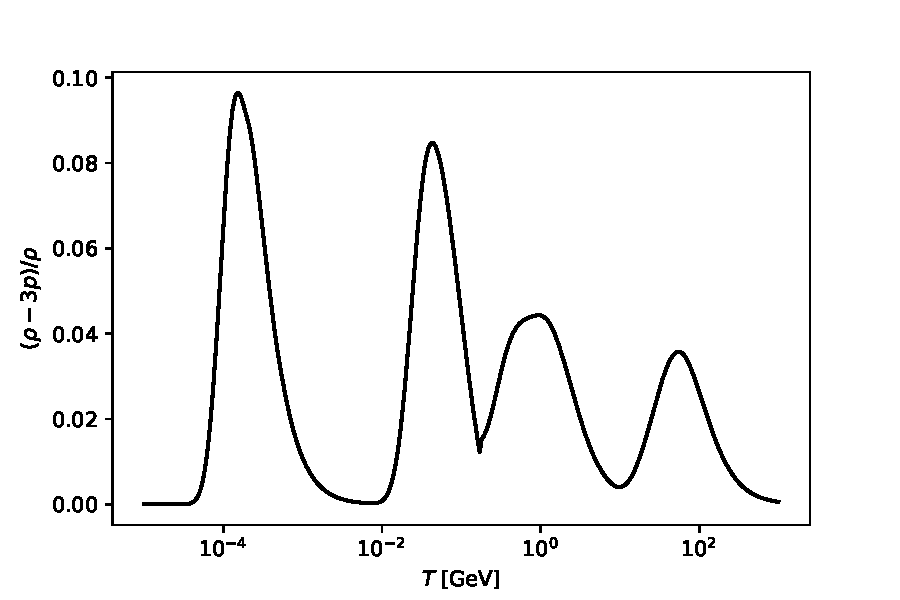
\includegraphics[scale=0.7]{figures/trace.pdf}% 图片在 Figures 文件夹中,注意修改尺寸大小 scale
\caption{能动量张量在宇宙早期随温度的演化。}% 图例
\label{trace}
\end{figure} % 第二章 正文,若要增加其他章节,复制一份修改即可,注意更改章节序号。
%\include{tex/chap3} % 第三章,以此类推
\newpage
 \vspace{1.0cm}
\setcounter{section}{3}
\setcounter{subsection}{0}
\setcounter{equation}{0}
\setcounter{figure}{0}
\setcounter{table}{0}
\section*{\centerline {\hei \sanhao  第三章 \ \ \ \ 总结与展望}}
\label{3}
\vspace{0.5cm}

啊,终于快写完了! % 总结与展望,这里为第三章

\newpage
 \vspace{1.0cm}
 \vspace{0.5cm}
\setcounter{section}{4}
\renewcommand{\theequation}{A.\arabic{equation}}
\setcounter{subsection}{0}
\setcounter{equation}{0}
\setcounter{figure}{0}
\setcounter{table}{0}
\section*{\centerline {\hei \sanhao  附录A\quad 附录标题}}
\label{A}

主线任务已达成,在附录中对相关内容做进一步补充和讨论吧。(字数还不够附录凑……)

\subsection*{\sihao \hei A.1\quad 通过 GitHub 写论文}
\label{A.1}

推荐使用 VS code 编辑和排版论文(安装 LaTeX Workshop
插件),
通过 SumatraPDF 快速浏览 PDF 文件,
同时在 GitHub 上建立一个私人仓库进行版本控制。
具体操作方式,请自行搜索,有时间我再补充。 % 附录

\newpage
\label{bib}
\renewcommand\refname{参考文献}
\setlength{\baselineskip}{14pt}
\bibliographystyle{unsrt}
\bibliography{tex/references} % 注意是 BibTeX 格式,文件名为 references.bib

\newpage
\newpage
\vspace{1.0cm}
\section*{\centerline {\hei \sanhao  在校期间发表的论文、科研成果等}}
\label{work}
%\setlength{\baselineskip}{19pt}  \centerline{\hei \sanhao 在校期间发表的论文、科研成果等}
\vspace{0.5cm}

\begin{enumerate}
\item 在这里列举已发表的文章。若是提交盲审的论文,则只需要说明在什么期刊发表了多少篇文章。
\end{enumerate} % 在校期间发表的论文、科研成果等
\newpage
\newpage
\vspace{1.0cm}
\section*{\centerline {\hei \sanhao 致\quad 谢}}
\label{acknowlegement}
\vspace{0.5cm}

首先,感谢不知其名的原作者制作的这份模板,令我顺利地完成了硕士论文的写作。若有人知晓原作者的个人信息还请告知,我会正式征求他的同意,并署名。

其次,感谢岁月静好的研究生生活和所有温暖的人们。

最后,祝各位毕业生答辩顺利,前程似锦。


\rightline{}

\rightline{陈\ \ \ 华}

\rightline{2020年12月28日}

\rightline{于温暖的图书馆} % 致谢

\end{document}! 就是主要文件,只需编译它即可。
至于目录、引言、正文、参考文献等内容则分别放在 \verb!\include{/tex/}! 目录下,
然后在 \verb!\documentclass[12pt,a4paper]{article}
\usepackage{psfig,epsfig,graphicx,epstopdf}
\usepackage[UTF8]{ctex}
\usepackage{url}
\usepackage{IEEEtrantools}
  \usepackage{amsmath}
  \usepackage{amssymb}
  \usepackage{float}

% 由于论文一般比较长,为了方便查看,可以选择只编译 \includeonly{} 中的文件。
%\includeonly{tex/abstract,tex/chapter1,tex/chapter2,tex/appendix,tex/references,tex/toc}

\usepackage{indentfirst}
\usepackage[normal,footnotesize]{caption2}%%normal表示标题文本的格式是不足一行居中,多于左对齐;small是指标题号(如图..,表..)的字体大小。
\usepackage[sort]{cite}
\usepackage[top=3.9cm,bottom=3.5cm,left=2.8cm,right=3cm,headheight=1.2cm,footskip=0.8cm]{geometry}
\usepackage[colorlinks,linkcolor=black,anchorcolor=blue,citecolor=green]{hyperref}
\usepackage{pdfpages} % 插入pdf

%%%%%%%%%%%%%%%%%%%%%%%%
% 为了区分中文句号“。”和数学符号“o”,一般将其转换成英文句点“.”。
\catcode`\。=\active
\newcommand{。}{.}
%%%%%%%%%%%%%%%%%%%%%%%%

\makeatletter
\newcommand{\rmnum}[1]{\romannumeral #1}
\newcommand{\Rmnum}[1]{\expandafter\@slowromancap\romannumeral #1@}
\makeatother

%\textwidth=16.5cm
%\textheight=21.8cm
%\textwidth 14.3cm
%\textheight 19.9cm
%\oddsidemargin 1.2cm
%\oddsidemargin 1.2cm
%\evensidemargin 1.3cm
%\topmargin 0.3cm
%\headsep 25pt
%\hoffset=-28pt
%\voffset=-1.8cm
\def\baselinestretch{1.25}
\renewcommand{\theequation}%
  {\arabic{section}.\arabic{equation}}
  \renewcommand{\theequation}
  {\arabic{section}.\arabic{equation}}
\renewcommand{\thefigure}
  {\arabic{section}.\arabic{figure}}
\renewcommand{\thetable}
  {\arabic{section}.\arabic{table}}


\newcommand{\song}{\CJKfamily{song}} % 宋体 (Windows自带simsun.ttf)
\newcommand{\fs}{\CJKfamily{fs}} % 仿宋体 (Windows自带simfs.ttf)
\newcommand{\kai}{\CJKfamily{kai}} % 楷体 (Windows自带simkai.ttf)
\newcommand{\hei}{\CJKfamily{hei}} % 黑体 (Windows自带simhei.ttf)
\newcommand{\li}{\CJKfamily{li}} % 隶书 (Windows自带simli.ttf)
\newcommand{\you}{\CJKfamily{you}} % 幼圆 (Windows自带simyou.ttf)

\newcommand{\chuhao}{\fontsize{42pt}{\baselineskip}\selectfont} % 字号设置
\newcommand{\xiaochuhao}{\fontsize{36pt}{\baselineskip}\selectfont} % 字号设置
\newcommand{\yichu}{\fontsize{32pt}{\baselineskip}\selectfont} % 字号设置
\newcommand{\yihao}{\fontsize{26pt}{\baselineskip}\selectfont} % 字号设置
\newcommand{\erhao}{\fontsize{21pt}{\baselineskip}\selectfont} % 字号设置
\newcommand{\xiaoerhao}{\fontsize{18pt}{\baselineskip}\selectfont} % 字号设置
\newcommand{\sanhao}{\fontsize{15.75pt}{\baselineskip}\selectfont} % 字号设置
\newcommand{\sihao}{\fontsize{14pt}{\baselineskip}\selectfont} % 字号设置
\newcommand{\xiaosihao}{\fontsize{12pt}{\baselineskip}\selectfont} % 字号设置
\newcommand{\wuhao}{\fontsize{10.5pt}{\baselineskip}\selectfont} % 字号设置
\newcommand{\xiaowuhao}{\fontsize{9pt}{\baselineskip}\selectfont} % 字号设置
\newcommand{\liuhao}{\fontsize{7.875pt}{\baselineskip}\selectfont} % 字号设置
\newcommand{\qihao}{\fontsize{5.25pt}{\baselineskip}\selectfont} % 字号设置
%%%%%%%%%%%%%%%%%% 页眉与页脚 %%%%%%%%%%%%%%%%%%%%%%%%%%%%%%%%%%
\usepackage{fancyhdr,graphicx}
\newsavebox{\mygraphic}
\sbox{\mygraphic}{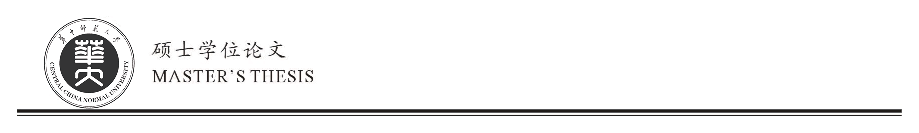
\includegraphics{logo.eps}}
\pagestyle{fancy}
\fancyhead{} % clear all header fields
\fancyhead[L]{\usebox{\mygraphic}}
\fancyfoot{} % clear all footer fields
\fancyfoot[C]{---\thepage---}
\renewcommand{\headrule}{%
\makebox[0pt][l]{\rule[0\baselineskip]{\headwidth}{0pt}}%
\rule[0\baselineskip]{\headwidth}{0pt} }

 %\renewcommand{\footrulewidth}{0.1pt}
 %\renewcommand{\headwidth}{\textwidth}


\begin{document}
\renewcommand{\refname}{\hei \sanhao 参考文献}
%%%%%%%%%%%%%%%%%%%%%%%%%%%%%%%%%%%%%%%%%%%%%%%%%%%%%%%%%%%%%%
%\
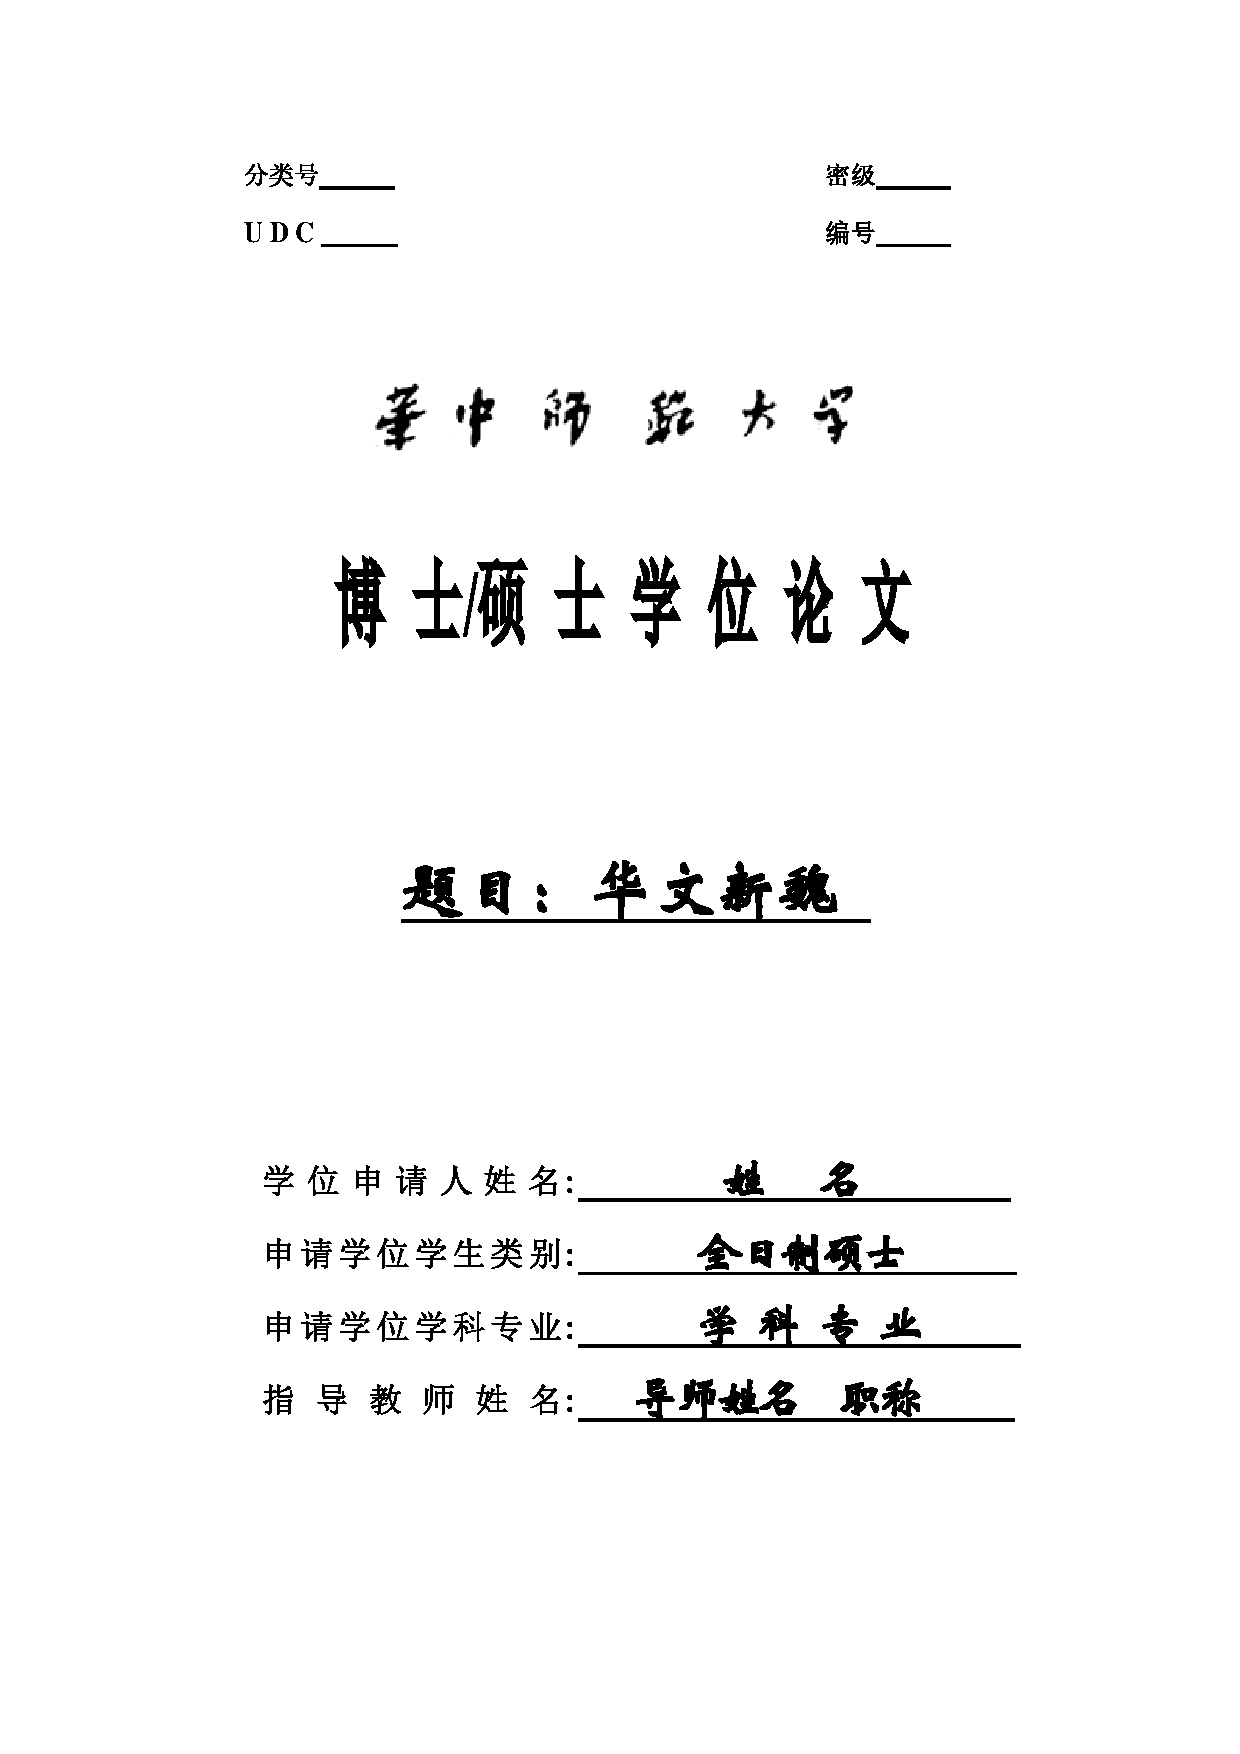
\includepdf{ccnu-cover.pdf} % 华师论文封面,在 ccnu-cover.doc 中修改,然后另存为 pdf 格式,替换掉模板
% 以下部分在 tex 文件夹中修改添加
% 标题页与授权页若不方便使用电子签名,可以先打印出来,签名后,扫描成 pdf 文件,按上述方法插入 tex 中
%%%%%%%%%%%%%%%%%%%% Chinese Cover %%%%%%%%%%%%%%%%%%%%%%%%%%%%%%%%%%%%%%%%%%%%
%\begingroup
%fancyfoot{} % clear all footer fields
%\thispagestyle{empty} %\markleft{\usebox{\mygraphic}}
\fancyfoot{}
\renewcommand{\thepage}{}
\begin{center}

%\hbox{} \vspace*{\fill}
\vspace*{2cm}
{\hei\yihao{{{\fontsize{28pt}{\baselineskip}\selectfont 硕士学位论文}}}}\\

\vspace*{2cm}

{\erhao \bf \hei 文章标题}\\


\vspace*{2.5cm}

\begin{huge}
\begin{center}
\begin{tabular}{cl}
  \xiaoerhao{\bf \hei 论文作者:}& \xiaoerhao{姓名} \\
  \xiaoerhao{\bf \hei 指导教师:}& \xiaoerhao{导师姓名\ 职称} \\
  \xiaoerhao{\bf \hei 学科专业:}& \xiaoerhao{专业名称} \\
  \xiaoerhao{\bf \hei 研究方向:}& \xiaoerhao{研究方向} \\
\end{tabular}
\end{center}
\end{huge}

\vspace*{3.5cm}

{\hei\xiaoerhao 华中师范大学物理科学与技术学院}

\vspace*{.5cm}

{\hei\xiaoerhao 2020年12月(修改时间)}

\vspace{\fill}
\end{center}

\newpage
%\endgroup

%%%%%%%%%%%%%%%%%%%% Second Cover %%%%%%%%%%%%%%%%%%%%%%%%%%%%%%%%%%%%%%%%%%%%
\newpage
%\begingroup
 \fancyfoot{} % clear all footer fields
%\thispagestyle{empty} %取消当前页码
\renewcommand{\thepage}{cover.en}
\begin{center}
%\hbox{} %\vspace*{\fill}

 \textbf{\xiaoerhao\bf \hei  论文英文标题}\\

 \vspace*{1.5cm}

{\large \sl A Thesis\\
\vspace*{0.4cm}
Submitted in Partial Fulfillment of the Requirements \\
\vspace*{0.4cm}For the Master's Degree in Astrophysics\\}

\vspace*{2cm}

{\normalsize\sanhao\hei\bf By}

\vspace*{0.4cm}

{\normalsize\sanhao\hei\bf 英文名}

\vspace*{0.4cm}

{\large \you \tt Postgraduate Program\\
\vspace*{0.4cm}
School of Physics and Technology\\
\vspace*{0.4cm} Central China Normal University\\}

\vspace*{2cm}

\textbf{\normalsize\sanhao\hei\bf Supervisor:
\hspace{1em}{\normalsize\sanhao\hei\bf  导师英文名}\hfill}

\vspace*{0.4cm}

\textbf{\normalsize\sanhao\hei\bf Academic Titles:
\hspace{1em}{\normalsize\sanhao\hei\bf 导师职称} \hfill}


\vspace*{0.5cm}

{\normalsize\sanhao \hfill Signature$\_ \_ \_ \_ \_ \_ \_ \_ \_ \_ \_ \_$}

\vspace*{0.3cm}

{\normalsize\sanhao \hfill Approved}

\vspace*{0.3cm}

{\normalsize\sanhao \hfill December, \hspace{0.5em}2020(修改时间)}

\vspace{\fill}

\end{center}
\newpage
%\endgroup
 % 标题页
%Authorization%%%%%%%%%%%%%%%%%%%%%%%%%%%%%%%%%%%%%%%%%%%%%%%%%%%
    \newpage
   %\thispagestyle{empty}
   \fancyfoot{} % clear all footer fields
    \begin{center}
    \title[\xiaoerhao {华中师范大学\\
    学位论文原创性声明和使用授权说明}
   \vspace{0.5cm}
    \parbox[t][1cm][c]{\textwidth}{ {\bf \sanhao \kai \centerline
    {原创性声明} } }
    \parbox[t][3cm][c]{\textwidth}{\xiaosihao
    \hspace{2em}本人郑重声明:所呈交的学位论文,是本人在导师指导下,独立
    进行研究工作所取得的研究成果。除文中已经标明引用的内容外,本论文不包含
    任何其他个人或集体已经发表或撰写过的研究成果。对本文的研究做出贡献的个
    人和集体,均已在文中以明确方式标明。本声明的法律结果由本人承担。}
    \parbox[t][2cm][c]{\textwidth}{\fontsize{12pt}{15pt}\selectfont
    \hspace{2em}\fs
    学位论文作者签名:
    \hspace*{3.3cm} 日期:\hspace{2em}年\hspace{2em}月\hspace{2em}日
    }

    \parbox[t][2cm][c]{\textwidth}{ {\sanhao \bf \kai \centerline
    {学位论文版权使用授权书} } }
    \parbox[t][3cm][c]{\textwidth}{\xiaosihao
    \hspace{2em}本学位论文作者完全了解学校有关保留、使用学位论文的规定,即:
    学校有权保留并向国家有关部门或机构送交论文的复印件和电子版,允许论文被查阅
    和借阅。本人授权华中师范大学可以将本学位论文的全部或部分内容编入有关数据库
    进行检索,可以采用影印、缩印或扫描等复制手段保存和汇编本学位论文。}
   \parbox[t][1.7cm][c]{\textwidth}{\fontsize{12pt}{15pt}\selectfont
   \hspace{2em}\fs
   学位论文作者签名:
   \hspace*{3.5cm}
   指导教师签名:}
   \parbox[t][1.8cm][c]{\textwidth}{\fontsize{12pt}{15pt}\selectfont
   \hspace{2em}\fs 日期:\hspace{2em}年\hspace{2em}月\hspace{2em}日
    \hspace*{2.3cm}日期:\hspace{2em}年\hspace{2em}月\hspace{2em}日
  \vspace{1.5cm}
}
 .\dotfill .
    \parbox[t][2cm][c]{\textwidth}{ {\fontsize{12pt}{18pt}\selectfont
    \hspace{2em}本人已经认真阅读"CALIS高校学位论文全文数据库发布章程",
    同意将本人的学位论文提交"CALIS高校学位论文全文数据库"中全文发布,
    并可按"章程"中的规定享受相关权益。同意论文提交后滞后:$\Box$半年;$\Box$一年;$\Box$二年发布。}}
   \parbox[t][1.5cm][c]{\textwidth}{\fontsize{12pt}{15pt}\selectfont
   \hspace{2em}\fs
   学位论文作者签名:
   \hspace*{3.5cm}
   指导教师签名:}
   \parbox[t][0.4cm][c]{\textwidth}{\fontsize{12pt}{15pt}\selectfont
   \hspace{2em}\fs 日期:\hspace{2em}年\hspace{2em}月\hspace{2em}日
    \hspace*{2.3cm}日期:\hspace{2em}年\hspace{2em}月\hspace{2em}日
    }
    \end{center} % 授权页
\pagenumbering{roman}
\newpage
 \vspace{1.0cm}
 \headsep=1.5cm
 \centerline{\hei \sanhao 摘\ \ \ \ \ 要}
 \label{zhaiyao}
\vspace{0.5cm}
 \pagestyle{fancy}
 \fancyfoot[C]{---\thepage---}

这是华中师范大学物理科学与技术学院\textbf{非官方}硕士学位论文 \LaTeX 模板(官方只有 Word 模板),
理论上适用于所有专业。
原作者未知,若有人知晓,还望告知,我将正式征求授权和为其署名。

考虑到有人可能不熟悉 \LaTeX,
以及模板的流传范围太过狭窄,
我对其稍加修改,
私自上传到~\href{https://github.com/ichenh/ccnu-latex}{GitHub}~网站。
其中,我补充了更详细的说明,
添加了中文句号转换成英文句点命令,
增加了华师官方要求的论文(存档)封面,
将过期的 Hua-Zhong Normal University 图标换成了新的 Central China Normal University,
以及展示了一些基本的 \LaTeX 范例。
更详细的 \LaTeX 命令可参考 \CTeX 开发小组翻译的《\href{http://mirrors.ibiblio.org/CTAN/info/lshort/chinese/lshort-zh-cn.pdf}{一份(不太)简短的 \LaTeX $\ 2\varepsilon$介绍}》,
我将电子版放在了补充材料文件夹中,
其中也附上了华师官方的学位论文写作要求。
请随意使用和修改模板,欢迎补充,如有错漏,
还请在 GitHub 上提交 issue 或 Pull Request。

另外,建议使用 \href{https://ctan.org/mirrors/mirmon#cn}{TeX Live} 编译软件以及它自带的 TeXworks 编辑软件。
具体步骤是:

\begin{itemize}
\item[1.] 修改论文封面:编辑根目录中的 \verb!ccnu-cover.doc! 文件,另存为 \verb!ccnu-cover.pdf!,覆盖原有文件。
\item[2.] 打开 \verb!main.tex! 文件,按如下顺序进行排版生成 \verb!main.pdf! 文件:XeLaTeX $\to$ BibTeX $\to$ XeLaTeX $\to$ XeLaTeX。
\item[3.] 论文写作:打开 tex 文件夹,修改相应文件(对应于论文的不同部分和章节。
若要增加新的章节,复制一份 \verb!chapter2.tex!,修改成 \verb!chapter3.tex!,
在 \verb!main.tex! 中的 \verb!\include{tex/chapter3}! 下方添加 \verb!\include{tex/chapter3}!。以此类推。
\item[4.] 重复第二步,生成新的 \verb!main.pdf! 文件。
\end{itemize}

整体思路很简单,
由于论文一般很长,放在一个文件里不好整理,
所以分成多个文件,最后导入同一个文件中编辑。
根目录中的 \verb!main.tex! 就是主要文件,只需编译它即可。
至于目录、引言、正文、参考文献等内容则分别放在 tex 目录下,
然后在 \verb!main.tex! 文件中通过 \verb!\include{}! 命令导入。

第二步中的 XeLaTeX 负责编译中文文本,BibTeX 是编译 \verb!.bib! 格式的参考文献。
若是使用了论文管理软件,可以选择导出为 \verb!.BibTeX! 文件,
覆盖 tex 文件夹下的 \verb!references.bib! 文件。
或者自己搜索相关文献的 BibTeX 引用格式,
将其复制到 tex 目录下的 \verb!references.bib! 文件中。
通过 BibTeX 编译出参考文献之后就只需要选择 XeLaTeX 编译,除非增加了新的文献。

\vspace{1cm} \noindent {\sihao \hei \textbf{关键词:}}华中师范大学;物理科学与技术学院;硕博士论文模板



\newpage %\vspace{1.5cm}
\headsep=0.7cm
\centerline{\bf \sanhao Abstract}
\label{abs}
\vspace{0.5cm}

Emmm...

\vspace{1cm} \noindent {\sihao \textbf{Keywords: }}CCNU; College of Physical Science and Technology; Tempolate of Doctoral or Master thesis % 摘要
\newpage
\pagestyle{fancy}
\thispagestyle{empty}
 %\fancyfoot{}
 \vspace{1.0cm}
 \centerline{\hei \sanhao 目\ \ \ \ \ 录}
\vspace{0.5cm} \label{content} \noindent
{\hei \xiaosihao 摘要 \dotfill \pageref{zhaiyao}}\\[0.2cm]
{\hei \xiaosihao ABSTRACT \dotfill \pageref{abs}}\\[0.2cm]
%{\hei \xiaosihao 目录\dotfill \pageref{content}}\\[0.2cm]
{\hei \xiaosihao 第一章\ \ \ \ 引言 \dotfill \pageref{1}}\\[0.2cm]
\hspace*{0.5cm} \ \  \ 1.1\ \  第一节\dotfill \pageref{1.1}\\
\hspace*{0.5cm} \ \  \ 1.2\ \  第二节\dotfill \pageref{1.2}\\[0.2cm] % 每章末尾添加 [0.2cm]
{\hei \xiaosihao 第二章\ \ \ \ \LaTeX 举例 \dotfill \pageref{2}}\\[0.2cm]
\hspace*{0.5cm} \ \  \ 2.1\ \  宇宙学标准模型\dotfill \pageref{2.1}\\
\hspace*{0.5cm} \ \  \ 2.2\ \  粒子物理标准模型\dotfill \pageref{2.2}\\[0.2cm]
{\hei \xiaosihao 第三章\ \ \ \ 总结与展望 \dotfill \pageref{3}}\\[0.2cm]
{\hei \xiaosihao 附录A\ \ \ \ 附录A \dotfill \pageref{A}}\\
\hspace*{0.5cm} \ \  \ A.1\ 通过 GitHub 写论文\dotfill \pageref{A.1}\\[0.2cm]
{\hei \xiaosihao 参考文献 \dotfill \pageref{bib}}\\[0.2cm]
{\hei \xiaosihao 在校期间发表的论文、科研成果等\dotfill \pageref{work}} \\[0.2cm]
{\hei \xiaosihao 致谢\dotfill \pageref{acknowlegement}} % 目录,需手动输入章节名和序号
\pagenumbering{arabic}

\newpage
\vspace{1.0cm}
\setcounter{section}{1}
\setcounter{equation}{0}
\setcounter{figure}{0}
\setcounter{table}{0}
\section*{\centerline {\hei \sanhao  第一章 \ \ \ \ 引言}}
\label{1}
\vspace{0.5cm}

要开始写论文了!

\subsection{\sihao \hei 第一节}
\label{1.1}

好累啊,先看个泡面番休息一下吧。

\subsection{\sihao \hei 第二节}
\label{1.2}

咦,到饭点了。 % 第一章 引言
% 注意更改序号!请自行验证。
\newpage
\vspace{1.0cm}
\setcounter{section}{2} % 章节序号
\setcounter{subsection}{0} % 小节序号
\setcounter{equation}{0} % 公式序号
\setcounter{figure}{0} % 图片序号
\setcounter{table}{0} % 表格序号
\section*{\centerline {\hei \sanhao  第二章 \ \ \ \ \LaTeX 举例}}
\label{2} % 引用标签
\vspace{0.5cm}


\subsection{\sihao \hei 宇宙学标准模型}
\label{2.1}

啊,只剩下一个月了,赶紧开始推导广义相对论~\cite{Einstein:1915ca, Einstein:1915by}。%引用文献

从爱因斯坦-希尔伯特作用量出发:
% 行间公式
\begin{align}
S=\frac{1}{16\pi G}\int d^{4}x\sqrt{-g}\left(R-2\Lambda\right)+\int d^{4}x\sqrt{-g}\mathcal{L}_{\mathrm{Matter}}\,, 
\label{EH}
\end{align}
其中,$G$表示引力常数,$R$是里奇标量,$\Lambda$是宇宙学常数,$\mathcal{L}_{\mathrm{Matter}}$是物质的拉式量。

BLABLA...

于是从作用量~\eqref{EH}~%引用公式
我们可以得到爱因斯坦场方程:
\begin{align}
R_{\mu\nu}-\frac{1}{2}Rg_{\mu\nu}+\Lambda g_{\mu\nu}=8\pi GT_{\mu\nu}\,.
\label{GR}
\end{align}
其协变导数表明它满足能量守恒定律$\nabla^{\mu}T_{\mu\nu}=0$。%行内公式

\subsection{\sihao \hei 粒子物理标准模型}
\label{2.2}

\begin{figure}[!htbp]
\centering
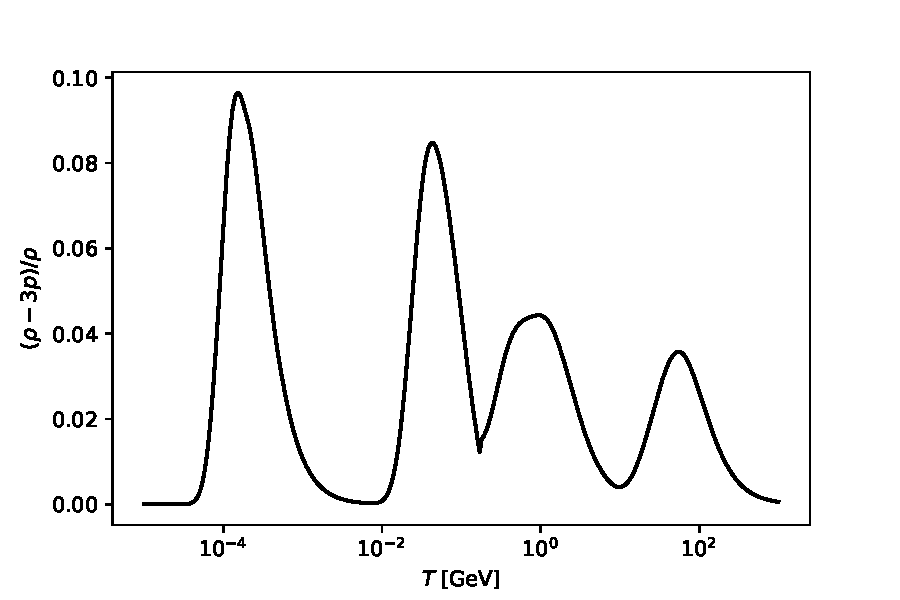
\includegraphics[scale=0.7]{figures/trace.pdf}% 图片在 Figures 文件夹中,注意修改尺寸大小 scale
\caption{能动量张量在宇宙早期随温度的演化。}% 图例
\label{trace}
\end{figure} % 第二章 正文,若要增加其他章节,复制一份修改即可,注意更改章节序号。
%\include{tex/chap3} % 第三章,以此类推
\newpage
 \vspace{1.0cm}
\setcounter{section}{3}
\setcounter{subsection}{0}
\setcounter{equation}{0}
\setcounter{figure}{0}
\setcounter{table}{0}
\section*{\centerline {\hei \sanhao  第三章 \ \ \ \ 总结与展望}}
\label{3}
\vspace{0.5cm}

啊,终于快写完了! % 总结与展望,这里为第三章

\newpage
 \vspace{1.0cm}
 \vspace{0.5cm}
\setcounter{section}{4}
\renewcommand{\theequation}{A.\arabic{equation}}
\setcounter{subsection}{0}
\setcounter{equation}{0}
\setcounter{figure}{0}
\setcounter{table}{0}
\section*{\centerline {\hei \sanhao  附录A\quad 附录标题}}
\label{A}

主线任务已达成,在附录中对相关内容做进一步补充和讨论吧。(字数还不够附录凑……)

\subsection*{\sihao \hei A.1\quad 通过 GitHub 写论文}
\label{A.1}

推荐使用 VS code 编辑和排版论文(安装 LaTeX Workshop
插件),
通过 SumatraPDF 快速浏览 PDF 文件,
同时在 GitHub 上建立一个私人仓库进行版本控制。
具体操作方式,请自行搜索,有时间我再补充。 % 附录

\newpage
\label{bib}
\renewcommand\refname{参考文献}
\setlength{\baselineskip}{14pt}
\bibliographystyle{unsrt}
\bibliography{tex/references} % 注意是 BibTeX 格式,文件名为 references.bib

\newpage
\newpage
\vspace{1.0cm}
\section*{\centerline {\hei \sanhao  在校期间发表的论文、科研成果等}}
\label{work}
%\setlength{\baselineskip}{19pt}  \centerline{\hei \sanhao 在校期间发表的论文、科研成果等}
\vspace{0.5cm}

\begin{enumerate}
\item 在这里列举已发表的文章。若是提交盲审的论文,则只需要说明在什么期刊发表了多少篇文章。
\end{enumerate} % 在校期间发表的论文、科研成果等
\newpage
\newpage
\vspace{1.0cm}
\section*{\centerline {\hei \sanhao 致\quad 谢}}
\label{acknowlegement}
\vspace{0.5cm}

首先,感谢不知其名的原作者制作的这份模板,令我顺利地完成了硕士论文的写作。若有人知晓原作者的个人信息还请告知,我会正式征求他的同意,并署名。

其次,感谢岁月静好的研究生生活和所有温暖的人们。

最后,祝各位毕业生答辩顺利,前程似锦。


\rightline{}

\rightline{陈\ \ \ 华}

\rightline{2020年12月28日}

\rightline{于温暖的图书馆} % 致谢

\end{document}! 文件中通过 \verb!\include{\include}! 命令导入。

第二步中的 XeLaTeX 负责编译中文文本,BibTeX 是编译 \verb!\include{.bib}! 格式的参考文献。
若是使用了论文管理软件,可以选择导出为 \verb!\include{.bib}! 文件,覆盖 \verb!\include{tex/references.bib}!
或者在 \href{}{inSPIRE} 中搜索相关文献,在该文献下方的 cite 选项中选择 BibTeX 格式,
复制到 \verb!\include{tex/references.bib}! 文件中。
通过 BibTeX 编译出参考文献之后就只需要选择 XeLaTeX 编译,除非增加了新的文献。

\vspace{1cm} \noindent {\sihao \hei \textbf{关键词:}}华中师范大学;物理科学与技术学院;硕博士论文模板



\newpage %\vspace{1.5cm}
\headsep=0.7cm
\centerline{\bf \sanhao Abstract}
\label{abs}
\vspace{0.5cm}

Emmm...

\vspace{1cm} \noindent {\sihao \textbf{Keywords: }}CCNU; College of Physical Science and Technology; Tempolate of Doctoral or Master thesis